\documentclass[conference]{IEEEtran}
% \documentclass[conference]{../sty/IEEEtran}

% *** CITATION PACKAGES ***
%
%\usepackage{cite}
% cite.sty was written by Donald Arseneau
% V1.6 and later of IEEEtran pre-defines the format of the cite.sty package
% \cite{} output to follow that of the IEEE. Loading the cite package will
% result in citation numbers being automatically sorted and properly
% "compressed/ranged". e.g., [1], [9], [2], [7], [5], [6] without using
% cite.sty will become [1], [2], [5]--[7], [9] using cite.sty. cite.sty's
% \cite will automatically add leading space, if needed. Use cite.sty's
% noadjust option (cite.sty V3.8 and later) if you want to turn this off
% such as if a citation ever needs to be enclosed in parenthesis.
% cite.sty is already installed on most LaTeX systems. Be sure and use
% version 5.0 (2009-03-20) and later if using hyperref.sty.
% The latest version can be obtained at:
% http://www.ctan.org/pkg/cite
% The documentation is contained in the cite.sty file itself.

% *** GRAPHICS RELATED PACKAGES ***
%
\ifCLASSINFOpdf
   \usepackage[pdftex]{graphicx}
  % declare the path(s) where your graphic files are
  % \graphicspath{{../pdf/}{../jpeg/}}
  % and their extensions so you won't have to specify these with
  % every instance of \includegraphics
  % \DeclareGraphicsExtensions{.pdf,.jpeg,.png}
\else
  % or other class option (dvipsone, dvipdf, if not using dvips). graphicx
  % will default to the driver specified in the system graphics.cfg if no
  % driver is specified.
   \usepackage[dvips]{graphicx}
  % declare the path(s) where your graphic files are
  % \graphicspath{{../eps/}}
  \graphicspath{ {./img/} }
  % and their extensions so you won't have to specify these with
  % every instance of \includegraphics
  % \DeclareGraphicsExtensions{.eps}
\fi
\graphicspath{ {./img/} }
% graphicx was written by David Carlisle and Sebastian Rahtz. It is
% required if you want graphics, photos, etc. graphicx.sty is already
% installed on most LaTeX systems. The latest version and documentation
% can be obtained at: 
% http://www.ctan.org/pkg/graphicx
% Another good source of documentation is "Using Imported Graphics in
% LaTeX2e" by Keith Reckdahl which can be found at:
% http://www.ctan.org/pkg/epslatex
%
% latex, and pdflatex in dvi mode, support graphics in encapsulated
% postscript (.eps) format. pdflatex in pdf mode supports graphics
% in .pdf, .jpeg, .png and .mps (metapost) formats. Users should ensure
% that all non-photo figures use a vector format (.eps, .pdf, .mps) and
% not a bitmapped formats (.jpeg, .png). The IEEE frowns on bitmapped formats
% which can result in "jaggedy"/blurry rendering of lines and letters as
% well as large increases in file sizes.
%
% You can find documentation about the pdfTeX application at:
% http://www.tug.org/applications/pdftex

% *** MATH PACKAGES ***
%
\usepackage{amsmath}
% A popular package from the American Mathematical Society that provides
% many useful and powerful commands for dealing with mathematics.
%
% Note that the amsmath package sets \interdisplaylinepenalty to 10000
% thus preventing page breaks from occurring within multiline equations. Use:
%\interdisplaylinepenalty=2500
% after loading amsmath to restore such page breaks as IEEEtran.cls normally
% does. amsmath.sty is already installed on most LaTeX systems. The latest
% version and documentation can be obtained at:
% http://www.ctan.org/pkg/amsmath


% *** SPECIALIZED LIST PACKAGES ***
%
\usepackage{algorithmic}
% algorithmic.sty was written by Peter Williams and Rogerio Brito.
% This package provides an algorithmic environment fo describing algorithms.
% You can use the algorithmic environment in-text or within a figure
% environment to provide for a floating algorithm. Do NOT use the algorithm
% floating environment provided by algorithm.sty (by the same authors) or
% algorithm2e.sty (by Christophe Fiorio) as the IEEE does not use dedicated
% algorithm float types and packages that provide these will not provide
% correct IEEE style captions. The latest version and documentation of
% algorithmic.sty can be obtained at:
% http://www.ctan.org/pkg/algorithms
% Also of interest may be the (relatively newer and more customizable)
% algorithmicx.sty package by Szasz Janos:
% http://www.ctan.org/pkg/algorithmicx


% *** ALIGNMENT PACKAGES ***
%
%\usepackage{array}
% Frank Mittelbach's and David Carlisle's array.sty patches and improves
% the standard LaTeX2e array and tabular environments to provide better
% appearance and additional user controls. As the default LaTeX2e table
% generation code is lacking to the point of almost being broken with
% respect to the quality of the end results, all users are strongly
% advised to use an enhanced (at the very least that provided by array.sty)
% set of table tools. array.sty is already installed on most systems. The
% latest version and documentation can be obtained at:
% http://www.ctan.org/pkg/array


% IEEEtran contains the IEEEeqnarray family of commands that can be used to
% generate multiline equations as well as matrices, tables, etc., of high
% quality.




% *** SUBFIGURE PACKAGES ***
%\ifCLASSOPTIONcompsoc
%  \usepackage[caption=false,font=normalsize,labelfont=sf,textfont=sf]{subfig}
%\else
%  \usepackage[caption=false,font=footnotesize]{subfig}
%\fi
% subfig.sty, written by Steven Douglas Cochran, is the modern replacement
% for subfigure.sty, the latter of which is no longer maintained and is
% incompatible with some LaTeX packages including fixltx2e. However,
% subfig.sty requires and automatically loads Axel Sommerfeldt's caption.sty
% which will override IEEEtran.cls' handling of captions and this will result
% in non-IEEE style figure/table captions. To prevent this problem, be sure
% and invoke subfig.sty's "caption=false" package option (available since
% subfig.sty version 1.3, 2005/06/28) as this is will preserve IEEEtran.cls
% handling of captions.
% Note that the Computer Society format requires a larger sans serif font
% than the serif footnote size font used in traditional IEEE formatting
% and thus the need to invoke different subfig.sty package options depending
% on whether compsoc mode has been enabled.
%
% The latest version and documentation of subfig.sty can be obtained at:
% http://www.ctan.org/pkg/subfig



% *** FLOAT PACKAGES ***
%
%\usepackage{fixltx2e}
% fixltx2e, the successor to the earlier fix2col.sty, was written by
% Frank Mittelbach and David Carlisle. This package corrects a few problems
% in the LaTeX2e kernel, the most notable of which is that in current
% LaTeX2e releases, the ordering of single and double column floats is not
% guaranteed to be preserved. Thus, an unpatched LaTeX2e can allow a
% single column figure to be placed prior to an earlier double column
% figure.
% Be aware that LaTeX2e kernels dated 2015 and later have fixltx2e.sty's
% corrections already built into the system in which case a warning will
% be issued if an attempt is made to load fixltx2e.sty as it is no longer
% needed.
% The latest version and documentation can be found at:
% http://www.ctan.org/pkg/fixltx2e


%\usepackage{stfloats}
% stfloats.sty was written by Sigitas Tolusis. This package gives LaTeX2e
% the ability to do double column floats at the bottom of the page as well
% as the top. (e.g., "\begin{figure*}[!b]" is not normally possible in
% LaTeX2e). It also provides a command:
%\fnbelowfloat
% to enable the placement of footnotes below bottom floats (the standard
% LaTeX2e kernel puts them above bottom floats). This is an invasive package
% which rewrites many portions of the LaTeX2e float routines. It may not work
% with other packages that modify the LaTeX2e float routines. The latest
% version and documentation can be obtained at:
% http://www.ctan.org/pkg/stfloats
% Do not use the stfloats baselinefloat ability as the IEEE does not allow
% \baselineskip to stretch. Authors submitting work to the IEEE should note
% that the IEEE rarely uses double column equations and that authors should try
% to avoid such use. Do not be tempted to use the cuted.sty or midfloat.sty
% packages (also by Sigitas Tolusis) as the IEEE does not format its papers in
% such ways.
% Do not attempt to use stfloats with fixltx2e as they are incompatible.
% Instead, use Morten Hogholm'a dblfloatfix which combines the features
% of both fixltx2e and stfloats:
%
% \usepackage{dblfloatfix}
% The latest version can be found at:
% http://www.ctan.org/pkg/dblfloatfix




% *** PDF, URL AND HYPERLINK PACKAGES ***
%
%\usepackage{url}
% url.sty was written by Donald Arseneau. It provides better support for
% handling and breaking URLs. url.sty is already installed on most LaTeX
% systems. The latest version and documentation can be obtained at:
% http://www.ctan.org/pkg/url
% Basically, \url{my_url_here}.

\usepackage[utf8]{inputenc}
\usepackage{amssymb}
\usepackage{algorithm}
\usepackage{multirow}
\newtheorem{definition}{Definition}
\renewcommand{\algorithmicrequire}{\textbf{Input:}}
\renewcommand{\algorithmicensure}{\textbf{Output:}}

\newcommand\alberto[1]{\textcolor{black}{#1}}

% *** Do not adjust lengths that control margins, column widths, etc. ***
% *** Do not use packages that alter fonts (such as pslatex).         ***
% There should be no need to do such things with IEEEtran.cls V1.6 and later.
% (Unless specifically asked to do so by the journal or conference you plan
% to submit to, of course. )


% correct bad hyphenation here
\hyphenation{op-tical net-works semi-conduc-tor}

\begin{document}
%
% paper title
% Titles are generally capitalized except for words such as a, an, and, as,
% at, but, by, for, in, nor, of, on, or, the, to and up, which are usually
% not capitalized unless they are the first or last word of the title.
% Linebreaks \\ can be used within to get better formatting as desired.
% Do not put math or special symbols in the title.
\title{Structural-temporal neighbourhoods of posts to characterize conversations in online forums}


% author names and affiliations
% use a multiple column layout for up to three different
% affiliations
\author{\IEEEauthorblockN{Alberto Lumbreras \\ Julien Velcin}
\IEEEauthorblockA{Laboratoire ERIC\\ Université de Lyon, France\\
alberto.lumbreras@univ-lyon2.fr\\
julien.velcin@univ-lyon2.fr}
\and
\IEEEauthorblockN{Bertrand Jouve}
\IEEEauthorblockA{FRAMESPA/IMT\\Université de Toulouse, France\\
jouve@univ-tlse2.fr}
\and
\IEEEauthorblockN{Marie Guégan}
\IEEEauthorblockA{Technicolor, France\\
marie.guegan@technicolor.com}}


% conference papers do not typically use \thanks and this command
% is locked out in conference mode. If really needed, such as for
% the acknowledgment of grants, issue a \IEEEoverridecommandlockouts
% after \documentclass

% for over three affiliations, or if they all won't fit within the width
% of the page, use this alternative format:
% 
%\author{\IEEEauthorblockN{Alberto Lumbreras\IEEEauthorrefmark{1},
%Bertrand Jouve\IEEEauthorrefmark{2},
%Marie Guégan\IEEEauthorrefmark{3}, 
%Julien Velcin\IEEEauthorrefmark{4}}
%\IEEEauthorblockA{\IEEEauthorrefmark{1}Technicolor, France\\Email: alberto.lumbreras@gmail.com}
%\IEEEauthorblockA{\IEEEauthorrefmark{2}Université de Toulouse; UT2; FRAMESPA/IMT,\\ 5 allée Antonio Machado, 31058 Toulouse, cedex 9\\
%Email: jouve@univ-tlse2.fr}
%\IEEEauthorblockA{\IEEEauthorrefmark{3}Technicolor\\975 Avenue des Champs Blancs\\35576 Cesson-Sevigné,\\France\\Email: marie.guegan@technicolor.com}
%\IEEEauthorblockA{\IEEEauthorrefmark{4}Laboratoire ERIC, Université de Lyon,\\ 5 avenue Pierre Mendès France, 69676, Bron\\France\\Email: julien.velcin@univ-lyon2.fr}}

% use for special paper notices
\IEEEspecialpapernotice{(Draft version: \today)}

% make the title area
\maketitle

% As a general rule, do not put math, special symbols or citations
% in the abstract
\begin{abstract}Social network analysis provides tools to analyse the global and the local structure of graphs when these graphs represent users interactions. In the context of online conversations, usually represented by trees, there is a lack of tools to analyse the local structure of these conversations. In this paper, we introduced two novel definitions of neighbourhood adapted to conversation trees. We analyse them in two Reddit forum and, finally, we show that they can successfully detect different types of conversationalists in online forums. 
\end{abstract}

% no keywords




% For peer review papers, you can put extra information on the cover
% page as needed:
% \ifCLASSOPTIONpeerreview
% \begin{center} \bfseries EDICS Category: 3-BBND \end{center}
% \fi
%
% For peerreview papers, this IEEEtran command inserts a page break and
% creates the second title. It will be ignored for other modes.
\IEEEpeerreviewmaketitle



\section{Introduction}
The interactions between users in online forums are often modelled as complex networks. As such, they can be studied from many levels, each of which is represented by a graph where vertices and edges may represent different things. The most studied graph is a graph where vertices represent users and edges represent interactions between users (a post from one user replying to a post from another user). From the point of view of the community, some typically analysed properties are the degree distribution, the clustering coefficient, density, or the diameter of the graph. From the point of view of the individual users, analyses are typically focused either on the centrality of users, on the community structure or in blockmodeling (groups of users that tend to interact with the same other groups) \cite{McCallum2007a}. Another common graph is a tree graph where vertices represent posts (or e-mails) and edges from one vertex to another indicate that the first is a reply to the second. Given the different discussion trees of a forum (a forest) the global analyses include depth distribution, branching factors, or even the time between two posts \cite{Bhatt2012, Gaumont2016,Dorat2007}. 

Studying discussion trees from the point of view of the users means, since trees are discussions, studying the user at a conversational level. Unfortunately, there is a lack of tools to perform an structural analysis of the conversation trees at a local level. In this paper, we propose to fill this gap through the concept of \textit{structural-temporal neighbourhood}.  


Our goal in this paper is two-fold: on the one hand, to illustrate how structural-temporal neighbourhoods can play the role of triads for conversation trees, in the sense that they show us the local structures or dynamics from which the bigger graph emerges. On the other hand, to show how structural-temporal neighbourhoods can be used for the detection of different types of conversationalists in online forums or any other type of online discussion that is representable by a tree structure (e.g.: e-mails).

The remaining of the paper is as follows. We first discuss about the convenience of the classic neighbourhood definition in dynamic graphs such as discussion trees. Then we introduce our two new definitions of structural-temporal neighbourhoods. To illustrate the kind of neighbourhoods that we obtain in a real data, we analyse two Reddit forums. Finally, we apply our time-based neighbourhood definition to detect clusters of users that tend to appear in the same neighbourhoods. We close the paper with some suggestions of future research.

\section{Discussion trees}
% Introduce el objeto y la nomenclatura
We represent a discussion thread by a tree graph $G=(V,E)$ where $V$ is a set of $n$ vertices representing the posts (also called messages or comments) and $E$ is a set of $n-1$ directed edges that say which posts replied to which post. Vertices have two attributes namely time and author. If for two given vertices $v_i,v_j$ there exists an edge  $e=(v_i, v_j) \in E$ then $v_j$ is called the \textit{parent} of $v_i$, denoted as $p(v_i)=v_j$. The \textit{root} of the tree is the only vertex with no parent, and corresponds to the post that starts the discussion. We say that two vertices $v_i,v_k$ are \textit{siblings} if and only if $p(v_i)=p(v_k)$. A vertex $v_l$ is an ancestor of a vertex $v_i$ and $v_i$ is descendant of $v_l$ if and only if $v_l$ is in the path from $v_i$ to the root. A \textit{leaf} is a post with no replies. A \textit{branch} is the path between a leaf and the root. Two vertices $v_i$ and $v_m$ are said to be \textit{neighbours} if either $p(v_i)=v_m$ or $p(v_m)=v_i$. The neighbours of a vertex $i$ are its parent and its children.

%The interactions like those found in an online forum can be modelled, at least, by two sort of graphs. On the one hand, we can create a graph where vertices represent individuals and an edges represent an interaction between two individuals. At the individual level, this graph is suitable for a large set of analysis concerning the centrality of users, the detection of communities, the detection of groups that tend to interact with the same other groups. At the community level we can analyse properties such as the density of the graph, the clustering coefficient or the degree distribution. On the other hand, we can create a separate tree graph for every discussion where posts are represented by the vertices and and edge from one vertex to another indicates that first post is a reply to the second. This allows to analyse things like patterns of time delay between posts \cite{Bhatt2012}.

%We can even mix different levels of representations to study the relationship between the properties and dynamics among the different levels \cite{Dorat2007}.

%Of course, we are not limited to the study of graphs and some studies take into account the content of the conversations, the cross-posting activity of users, and so forth \cite{Whittaker1998}

%Others: \cite{Gaumont2016}

\section{Structural neighbourhoods}\label{sec:structural}
Extending the classic definition of neighbourhood, we recall the definition of \textit{structural neighbourhood}\footnote{We coined the term \textit{structural} to differentiate if from the other neighbourhoods discussed in this paper.}:

\begin{definition}
Given a tree graph $G$, the \textit{structure-based neighbourhood} of radius $r$ of post $i$, denoted as $\mathcal{N}_i(r)$, is the induced graph composed by all the vertices that are at distance equal or less than $r$ from post $i$.
\end{definition}
% pros and cons
In the context of discussion threads, this definition has two limitations. First, the decision on whether to include some post in the neighbourhood is only based on the structural distance, and therefore two posts that are at distance $d\leq r$ are considered neighbours of $i$ regardless of the time when they were written although, in conversations, time plays an important role. Another consequence of looking only at the structure is that the number of possible neighbourhoods within a radius $r$ is infinite. This poses a problem when trying to categorize conversations since many conversations, while structurally different, can be considered semantically similar (e.g.: we might not want to put in different categories two structures representing, respectively, a post with 50 replies and another with 40).

\section{Structural-temporal neighbourhoods}\label{sec:temporal}
We propose two refinements of the structure-based neighbourhood to take into account the order and time at which posts are written. In the order-based definition, a new radius is set to include at most the $n$ closest posts in time.  In the time-based definition, the new radius is set to include all posts (in the structural-neighbourhood) until the first point where the conversation slows down. 


\begin{figure}
\centering
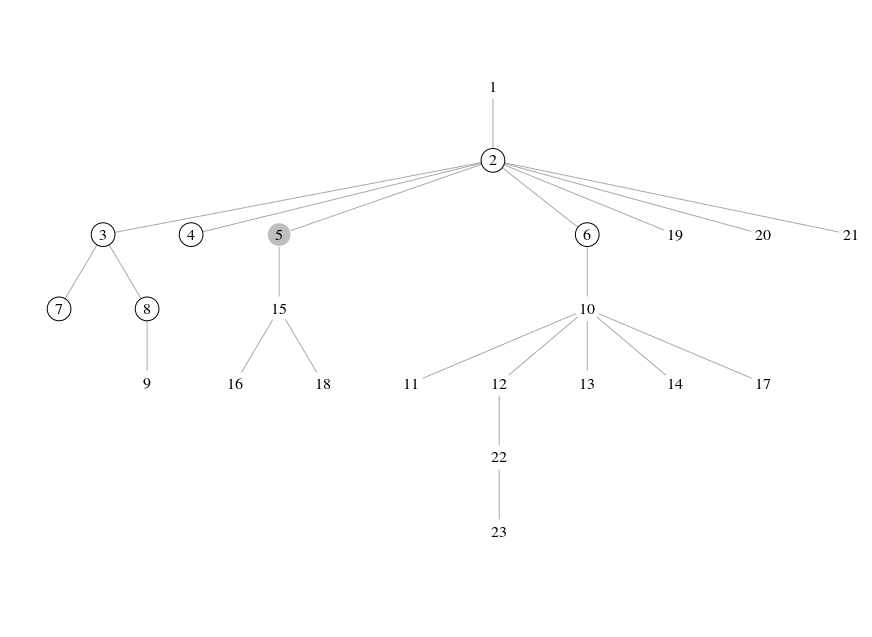
\includegraphics[width=0.45\textwidth]{order_neighbourhood}
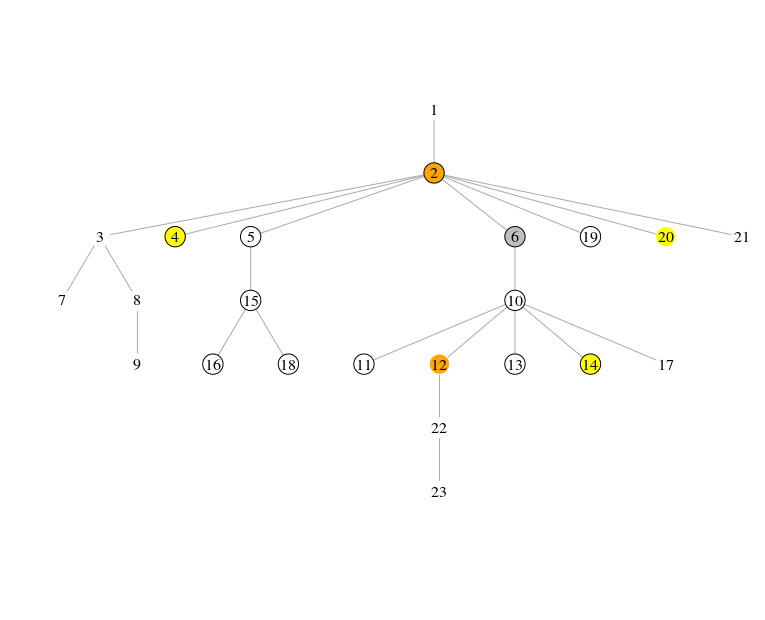
\includegraphics[width=0.45\textwidth]{breakpoints}
\caption{Illustration of order-based (top) and time-based (bottom) neighbourhoods. Grey nodes represent the ego post. Nodes with circles are those in the neighbourhood. Numbers indicate the order of the post. The order-based neighbourhood has parameters $r=3$, $n=6$. The time-based neighbourhood has parameter $r=3$. In the time-based neighbourhood, horizontal changepoints (yellow) and vertical changepoints (orange) represent posts that are temporally far from their predecessors (siblings or parents) and therefore set the limits of the neighbourhood.}
\label{fig:cutpoints}
\end{figure}
\subsection{Order-based}
\begin{definition}
Given an ordered tree graph $G$, the \textit{order-based neighbourhood} of radius $r$ and order $n$ of vertex $i$, denoted as $\mathcal{N}_{i}^O(r,n)$ is the induced subgraph from its structural neighbourhood $\mathcal{N}_{i}(r)$ composed by the $n$ vertices that are closest to $i$ in time and for which there exists a path to $i$ in $\mathcal{N}_{i}^O(r,n)$.  
\end{definition}
An example of order-based neighbourhood is given in Figure~\ref{fig:cutpoints}.
This definition has two advantages over the \textit{structural neighbourhood}. First, the temporal aspect of the conversation is better taken into account since the neighbourhood only includes posts that are not only near to $i$ in the structure but also in time. Second, the size of the neighbourhood has an upper bound of $min(|\mathcal{N}_i(r))|, n)$ thus making the space of possible neighbourhood structures finite. The main limitation of this definition is that the we have no \textit{a priori} criteria to choose the proper parameter $n$ other than making it small to capture only the local dynamic of the conversation around the post $i$.

\subsection{Time-based}
In order to take time explicitly into account, one might set fixed time-based boundaries for the neighbourhood and include only those posts whose timestamp $t_j$ is at distance less than $\tau$ from the ego post $i$, $|t_j-t_i|<\tau$. However, the pace at which posts are added to the conversation may be very different between conversation threads (and also within a thread) and we have no \textit{a priori} criteria for a proper choice of $\tau$. 

Rather than looking for a fixed time radius, we may instead decide it by looking at changes in the pace how new posts are added to the thread. In statistical analysis, a \textit{changepoint} in a sequence $x_1,...x_n$ is a point that comes from a different probability distribution than its precedent values. If sequences are timestamps, they are monotonic increasing, therefore the changepoints will correspond to sudden pauses in the conversation. In the following, we will differentiate \textit{horizontal changepoints}, that arise between siblings, from \textit{vertical changepoints}, that arise within a branch. We say that a sequence posts with timestamps $t_1,...,t_n$ belong to the same (vertical or horizontal) \textit{local dynamic} if there is no changepoint $t_i$ in the sequence such that $1 < i \leq n$. For the detection of changepoints we use the PELT algorithm \cite{Killick2012}\footnote{An implementation of this algorithm written by the authors themselves is available in the R library \texttt{changepoint}. We use their \texttt{cpt.meanvar} function.}. Now we can introduce our second definition of neighbourhood.
\begin{definition}
Given a tree graph $G$, the \textit{time-based neighbourhood} of radius $r$ of vertex $i$, denoted as $\mathcal{N}_{i}^T(r)$, is the maximal subgraph of the structural neighbourhood $\mathcal{N}_i(r)$ where all the vertices  belong to the same vertical and horizontal local dynamic as $i$.
\end{definition}
Note that we still have a radius parameter $r$ to guarantee that the resulting structure remains local even if no changepoint is detected near the post $i$. 

% Explain algorithm
Algorithm \ref{alg:temporal_neighbourhood} extracts time-based neighbourhoods of a given post according to the above definition. Since the changepoints only depend on the tree and not on the particular post we analyse, we previously detect the horizontal and vertical changepoints in the tree. In the case of multiple branches with some common posts, we consider that a common post is a vertical changepoint if it is a vertical changepoint in any of the branches. Once we have the changepoints, we can proceed with the algorithm. First, we extract the structural-neighbourhood. The time-based neighbourhood will be a subset of the later. Then, we look for horizontal and vertical changepoints, which mark the frontiers of the time-based neighbourhood. There are four possible cases:

\begin{itemize}
\item A \textit{vertical changepoint in the ancestors}: If the changepoint is in the path between the post and the root, then the changepoint started the new local dynamic to which the ego post belongs. Thus, we remove the ancestors of the changepoint, but not the changepoint itself.
\item A \textit{vertical changepoint in the descendants}: If the changepoint is a descendant then it started a new different dynamic and therefore we must remove the descendants of the changepoint and the changepoint itself. 
\item A \textit{horizontal changepoint either in the older siblings or in the ancestors}: If the changepoint is among the older siblings, then it started the horizontal dynamic to which the ego post belongs. Similarly, if the changepoint is among the ancestors, then every older sibling of the changepoint belongs to a previous local dynamic. In both cases, we remove the older siblings of the changepoint but not the changepoint itself.
\item A \textit{horizontal changepoint elsewhere}: In any other case, the horizontal changepoint starts a different local dynamic and therefore we remove its younger siblings and the changepoint. 
\end{itemize}
Any time a vertex is removed we also remove its descendants. $\mathcal{N}_i^T(r)$ is a connected induced subgraph of $\mathcal{N}_i(r)$.  If there are no changepoints in the structural neighbourhood, then $\mathcal{N}_i^T(r) = \mathcal{N}_i(r)$.

%Example
An example of time-based neighbourhood is given in Figure~\ref{fig:cutpoints} (right).

\begin{algorithm}[H]
\begin{algorithmic}
\REQUIRE Posts tree $G$, vertical changepoints, horizontal changepoints, ego post $i$, radius $r$
\ENSURE $\mathcal{N}_i^{T}(r)$: Time-based neighbourhood of $i$ at radius $r$
\STATE Compute structural neighbourhood $\mathcal{N}_i(r)$
\STATE ancestors $\leftarrow$  ancestors($i$) in $\mathcal{N}_i(r)$
\STATE older\_siblings $\leftarrow$ older\_siblings($i$) in $\mathcal{N}_i(r)$
\STATE dump $\leftarrow \varnothing$
\FOR{bp $\in$ vertical changepoints}
 \IF{bp $\in$ ancestors}
   \STATE dump $\leftarrow$ dump $\cup$ ancestors(bp)
 \ELSE
   \STATE dump $\leftarrow$ dump $\cup$ descendants(bp) $\cup$ bp
  \ENDIF
\ENDFOR
\FOR{bp $\in$ horizontal changepoints}
  \IF{bp $\in$ (older\_siblings $\cup$ ancestors)}
     \STATE dump $\leftarrow$ dump $\cup$ older\_siblings(bp)
   \ELSE
     \STATE dump $\leftarrow$ dump $\cup$ younger\_siblings(bp) $\cup$ bp
  \ENDIF
\ENDFOR
\STATE $\mathcal{N}_i^{T}(r) \leftarrow$ delete(dump\_posts $\cup$ descendants(dump\_posts)) from $\mathcal{N}_i(r)$
\end{algorithmic}
\caption{Extraction of time-based neighbourhood}
\label{alg:temporal_neighbourhood}
\end{algorithm}

\section{Neighbourhood colouring and pruning}\label{sec:colouring_pruning}
\subsection{Colouring}
Even if the structure contains some important information about the type of conversation, there is still some ambiguity left, and two similar neighbourhoods can represent very different types of conversation. We can easily reduce this ambiguity by assigning colours to vertices, which allows us to identify some relevant property of the post. 

In particular, we assign the following colours:

\begin{itemize}
\item \textit{Red}: ego post.
\item \textit{Orange}: other posts written by the author of ego. It allows to identify re-entries (when the same author participates several times in the discussion \cite{Backstrom2013})
\item \textit{Yellow}: parent of ego post and other posts written by the same author. It allows to identify, for instance, debates between the ego author (red and orange) and this other author (yellow). We have observed this phenomena in our data, and it is often the cause of long chains.
\item \textit{White}: root post. Differentiating the root post from the rest has been proven by previous research on online discussions. For instance, some types of users seem to get more replies than others when they initiate a thread (\cite{Himelboim2009,  Lumbreras2013}). Also, in terms of preferential attachment, root posts usually get more replies than the non-roots (\cite{Gomez2010, Gomez2012}).
\item \textit{Black}: none of the above.
\end{itemize}
Since some posts might correspond to several colours, we perform a sequential assignment of colours given by $\texttt{black, orange, red, yellow, white}$. 

We do not claim this choice of labels to be of universal. Indeed, other labellings might also give interesting results since they would look at conversations from new points of view (e.g.: a colour for leaf vertices, colours according to the post length, or colours to represent the sentiment of the post). 

\subsection{Pruning}
At this point, we can still find structures the only difference of which is that one of them has more leafs hanging from some of the nodes. Thus, we prune every neighbourhood by leaving a maximum of two consecutive siblings of the same colour and where neither of them has any children. The reason of setting the limit to two is that it is the minimum necessary to distinguish between \textit{zero}, \textit{one} and \textit{more than one} consecutive occurrences. In other words, we consider that the difference between one and zero replies to a post is relevant, but that five and six replies do not make any difference worth being represented.  Moreover, this choice encourage smaller structures, which allows the computation of isomorphisms (Section~\ref{sec:extraction}) even in real time.  

\section{Application to Reddit forums}


Our data consists of two different forums of Reddit, namely the Podemos dataset \footnote{https://www.reddit.com/r/podemos} and the Game of Thrones dataset\footnote{https://www.reddit.com/r/gameofthrones}. The Podemos forum was conceived in March 2014 as a tool for internal democracy, and forum members used it to debate ideological and organizational principles that were later formalized in their first party congress hold in Madrid on October 18th and 19th, 2014. Nowadays, its members use it mainly to share and discuss about political news. The Game of Thrones forum is a casual discussion forum about the Game of Thrones TV series.
The Podemos dataset contains 75,000 posts corresponding to 4,262 threads written by 9,160 users between April 25th and October 20th, 2014. The Game of Thrones dataset contains 75,000 posts corresponding to 5,862 threads written by 18,907 users.

\subsection{Neighbourhood extraction}\label{sec:extraction}
As a previous step for all further analysis, we extracted the structure-based ($r=2$), the order-based ($r=2, n=4$) and the time-based ($r=2$) neighbourhood around every post for the two forums. 

For each method (structure-based, order-based or time-based) we extract the neighbourhood around every post of a forum as follows. A new label is assigned to every neighbourhood structure the first time it is detected. For every post, we extract its neighbourhood, colour and prune it (Sections~\ref{sec:structural} and \ref{sec:temporal}). Then we check whether it is isomorphic to some of the $n$ neighbourhoods that we have already seen. If this is the case, then the current neighbourhood is given the same label than the neighbourhood that we already saw. Otherwise we create a new label for the current neighbourhood. The set of neighbourhoods found and their labels constitutes a \textit{dictionary}. 

Once the six extractions are finished, we merge the dictionaries into a global one and re-label the neighbourhoods by frequency (1 for the most frequent and so forth). Figure \ref{fig:dictionary} shows some frequent neighbourhoods that will be discussed later.

% Computational cost
In the worst case, where every post has a unique neighbourhood, every extracted neighbourhood should be compared against every neighbourhood that already appears in the dictionary before concluding that it needs a new entry. In this case, the computational cost of this operation is $\mathcal{O}(n^2)$ where $n$ is the number of posts. In practice, however, the bigger the number of posts processed, the less likely we go through all the dictionary without finding an isomorphism. Moreover, if we keep the dictionary sorted by frequency, a large number of neighbourhoods will find an isomorphism among the first neighbours of the dictionary. 

\subsection{Comparing neighbourhood methods}
In this section we compare different aspects of the three methods, namely (a) the size and frequency distribution of the neighbours for each method, (b) the discrepancies between methods when they extract the neighbourhood of a same post.

\subsubsection{Size and frequency distribution}
We detected in the whole dataset 3,791 different structure-based neighbourhoods, 174 different order-based and 1,488 different time-based, which means that the structure-based captures a much wider set of structures. Of course, this is not necessarily an advantage since these extra structures may be just spurious and only occur a very small number of times. Indeed, Figure~\ref{fig:census_distributions} shows that around half of the time-based neighbourhoods (41\%) and the structure-based neighbourhoods (60\%) occur only once, while the number of neighbourhoods that appear more than 100 times (among 150,000 posts) is similar for the three types of neighbourhood. To cover 95\% of the posts we need 623 structure-based neighbourhoods, 40 order-based and 155 time-based. 
 
% Why order-based is not good enough
The main reason why the frequency of the order-based neighbourhoods decays faster is that the most frequent neighbourhood (id 1) is much more frequent (upper-left red point in the left plot of figure \ref{fig:census_distributions}) than the most frequent time-based neighbourhood. This is the main handicap of the order-based neighbourhood since, as we will see later, it avoids finding richer structures. Table~{\ref{tab:table}} shows the most frequent neighbourhoods for the three methods in each forum. The results are quite sensitive to the choice of the neighbourhood. Note that the order-based detects less differences among the most frequent neighbourhoods in both forums. Besides, it seems that when the time-based detects the neighbourhood 4, the structure-based detects the neighbourhood 7. This illustrate the effect of the changepoint: the presence of an horizontal changepoint in 7 (many posts replying to the root) converts it, from the point of view of the time-based neighbourhood, to a 4, which indicates that the ego has at most two siblings in the same period of time.

\begin{figure*}
\centering
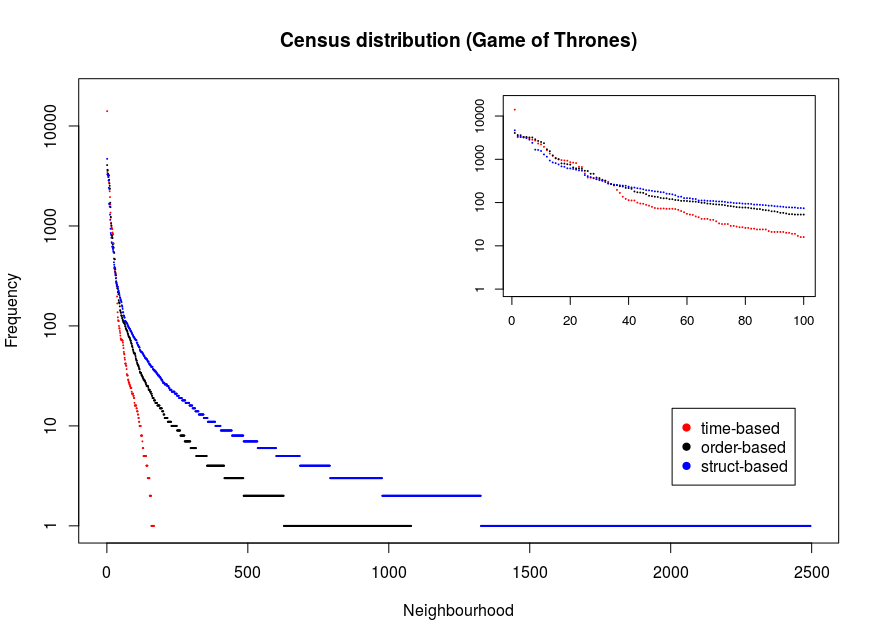
\includegraphics[width=0.5\textwidth]{compare_census_distribution_gameofthones}%
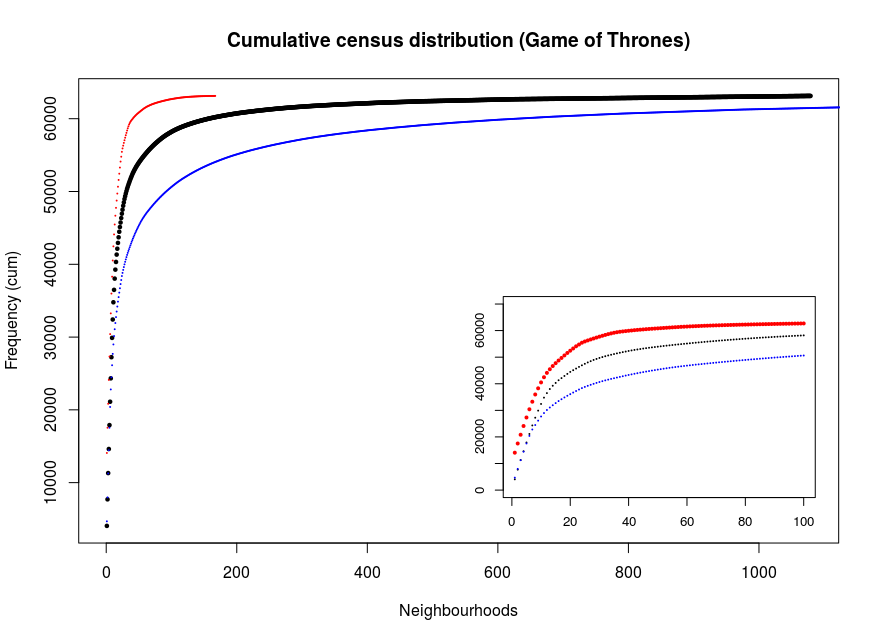
\includegraphics[width=0.5\textwidth]{compare_census_distribution_gameofthones_cum}
\caption{Comparison of census distributions with order-based and time-based neighbourhoods.}
\label{fig:census_distributions}
\end{figure*}

%\begin{figure}
\begin{table}
 \begin{center}
   \tabcolsep = 0.8\tabcolsep
   \begin{tabular}{|rr|rr|rr|}
      \hline
      \multicolumn{2}{|c|}{struct-based} & \multicolumn{2}{|c|}{order-based} &  \multicolumn{2}{|c|}{time-based} \\
      %\hline
     	 POD & GOT 						& POD & GOT 		& POD & GOT\\
   \hline \hline
     7 (9.6)	& 7 (7.4)   		&  		1 (25.2) & 1 (25.2) &  4 (9.0) & 4 (6.4)\\    
     3 (16.5)& 9 (12.6)   	&  	3 (32.1) & 3 (32.1) &  8 (17.2) & 8 (12.2)\\ 
     2 (23.1)& 3 (17.8)   	&  	2 (38.8) & 2 (38.8) &  2 (25.3) & 2 (17.9)\\ 
     20 (27.8)& 11 (22.9)   &  	13 (45.3) & 13 (45.3) &  3 (31.2) & 9 (23.2)\\    
     4 (31.1)& 5 (27.8)   	&  	4 (50.1) & 4 (50.1) &  10 (36.6) & 14(28.4)\\ 
     13 (34.1)& 2 (32.3)   	&  	18 (54.7) & 18 (54.7) &  14 (41.8) & 11(33.5)\\ 
     6 (36.9)& 12 (36.1)   	&  	6 (58.9) & 6 (58.9) &  6 (45.8) & 10(38.5)\\    
     5 (39.4)& 27 (38.8)   	&	  	12 (65.5) & 10 (62.8) &  15 (48.9) & 5 (43.1)\\ 
     15 (41.9)& 4 (41.4)   	&  	16 (68.5) & 12 (65.5) &  19 (51.5) & 6 (47.4)\\  
     12 (43.7)& 6 (43.9)   	&  	5 (70.6) & 16 (68.1) &  5 (53.9) & 3 (51.3)\\    
     21 (45.3)& 21 (45.9)   	&  	17 (72.8) & 5 (70.7) &  7 (55.9) & 25(55.1)\\ 
     30 (46.9)& 15 (47.7)   	&  	23 (75.5) & 17 (72.8)&  16 (57.6) & 15(57.8)\\ 
     16 (48.4)& 13 (49.2)   	&  	31 (76.1) & 23 (74.5)&  36 (59.4) & 12(60.2)\\    
     39 (49.8)& 20 (50.6)   	&  	19 (77.5) & 31 (76.1) &  25 (61.2) & 7 (62.2)\\ 
     44 (51.2)& 30 (51.9)   	&  	22 (79.0) & 19 (77.5) &  21 (62.6) & 21(63.9)\\ 
     8 (52.4)& 22 (53.1)   	&	  	24 (80.3) & 22 (78.9) &  34 (63.9) & 19(65.5)\\    
     22 (53.3)& 43 (54.2)   	&  	26 (81.5) & 24 (80.3) &  38 (65.1) & 17(66.7)\\ 
     51 (54.2)& 8 (55.2)   	&  	29 (82.7)& 26 (81.5) &  23 (66.4) & 36(68.0)\\          
   \hline
   \end{tabular}
\label{tab:table}
 \end{center}
 \caption{Most frequent neighbourhoods (and cummulative frequence) for the three methods if Podemos (POD) and Game of Thrones (GOT) forums.}
\end{table}
%\end{figure}

\subsubsection{Discrepancies}
The divergent number of non-isomorphic neighbourhoods between structure-based, order-based and times-based methods suggests that some neighbourhoods, for instance, time-based, might be systematically mapped to the same neighbourhoods in order-based. Or similarly, that some structure-based neighbourhoods are systematically mapped into the same time-based neighbourhoods. Figure~\ref{fig:confusion} gives a general overview of these mappings. The left figure shows, for every post, its time-based neighbourhood and its order-based neighbourhood, while the right figure shows the time-based and the structure-based. The points in the diagonal correspond to posts that have been assigned the same neighbourhood by the two compared methods. 

The diagonal of the time-based / order-based plot contains 36\% of the posts. The diagonal of the structure-based / time-based plot contains 40\% of the posts. For the order-based / struct-based (not shown) there are 41\% of the posts in the diagonal. In general, the structures with a bigger agreement are among the most frequent. This is probably due to the fact that a high amount of threads are small and therefore there is less room for discrepancy. There is a 30.75\% of the posts that are assigned the same neighbourhood structure by the three methods. 

Rather than looking at where the methods agree, it is even more interesting to see where they disagree, since this will reveal whether one of the methods is incapable of detecting some interesting conversational structure. In Figure~\ref{fig:confusion} some horizontals lines can be spotted specially in the lower part of the plots. These correspond to posts with different time-based neighbourhoods that are assigned the same order-based neighbourhood (left), and different time-based neighbourhoods that are assigned the same order-based neighbourhood (right). Looking for the order-based neighbourhoods that have a correspondence with a larger set of time-based neighbourhoods, we detect that these correspond to neighbourhoods 1 (77 different time-based) and 50 (57 different time-based), 17 and 18. Looking for the time-based neighbourhoods that have a correspondence with a larger set of structure-based neighbourhoods, we detect that these are neighbourhoods 10, 4, 8, 19, 14.

% Wrap-up
In retrospective, these results are not surprising. What we see is simply that structures that are often captured by one method collapse into another single structure when another method with a smaller space of structures is used. Yet, the three methods mostly agree when they find a frequent neighbourhood. But this might be due to the fact that simpler motifs tend to be in shorter threads, where there is no room for two neighbourhood methods to detect a different structure.

\begin{figure*}
\centering
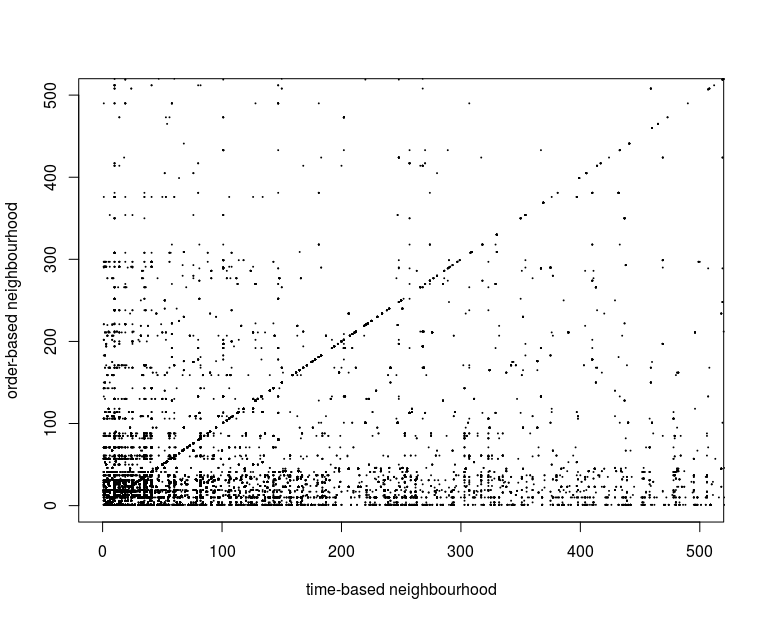
\includegraphics[width=0.5\textwidth]{confusion_time_order}%
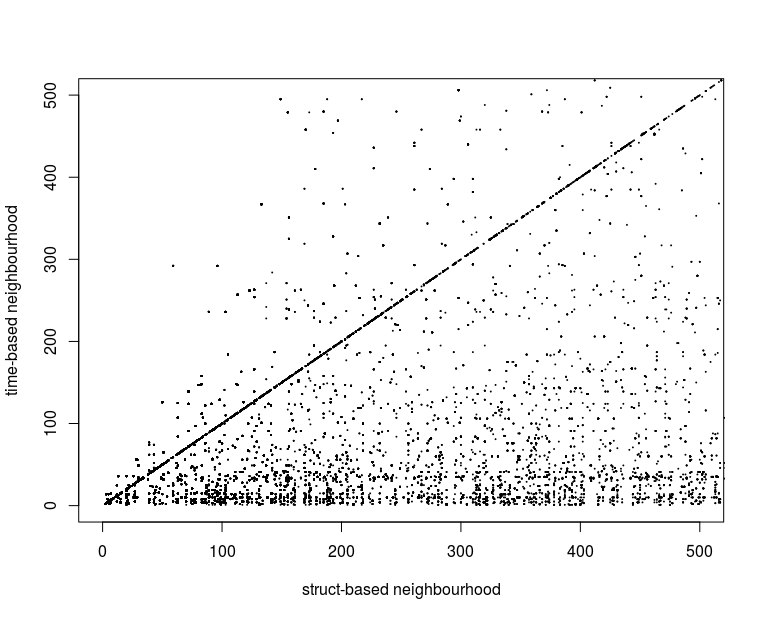
\includegraphics[width=0.5\textwidth]{confusion_struct_time}
\caption{Neighbourhood of posts from the point of view of order-based and time-based. Neighbourhoods with the same label in the order-based and the time-based axes are isomorphic. The points in the diagonal correspond to posts to whom the two methods assign exactly the same neighbourhood. Horizontal rows of points correspond to posts that are assigned many different time-based neighbourhoods but the same single order-based neighbourhood.}
\label{fig:confusion}
\end{figure*}



It is clear from the this analysis that the order-based does not do a good job on capturing all the richness of the conversational structures due to the dominance of neighbourhood 1. There are two other reasons to choose the time-neighbourhood over the structure based. First, the time-based has less spurious structures, covering 95\% of posts with 155 neighbourhoods, against the 623 neighbours necessary to cover that amount with the structure-based. Second, the time-based neighbourhood has more grounded criteria to decide where the neighbourhood ends, while the structure-based has no criteria at all.

\subsection{Conversation-based clustering of users}
In this section, we apply the time-based neighbourhoods to cluster users in the Podemos dataset based on the neighbourhoods of their posts. Our intuition is that some users like participating in some kind of discussion rather than other. Certainly, most part of the information necessary to understand the nature of a discussion in in its textual content. However, due to the huge diversity of topics, vocabulary, and the difficulty of current algorithms to capture the language subtleties such as humour, irony, or context, we turn our attention towards the structure of the discussions, which can also contain some information. We work under the  hypothesis that the structural-neighbourhoods in which a user post in embedded reflect the kind of conversation in that part of the thread. 

Our dataset contains a set of 100 \textit{active users} who wrote more than 100 posts. For those users, we create an initial feature matrix $U\times N$ where $U$ is the number of users and $N$ is the number of neighbourhoods in the dictionary, and where the the position $(u,n)$ is a counter of the number of times that a post written by user $u$ has a neighbourhood isomorphic to $n$. We drop those feature columns that are zero for every user (these are neighbourhoods seen only around posts of users with low-level activity). To make the feature vector of a user independent on the number of posts, we transform the counts into percentages. And since some features have much higher percentages than others for most users, we scale and normalize the matrix so that every feature has mean 0 and variance 1. To avoid non-significant scores, we remove also the feature column corresponding to neighbourhoods that have a frequency less than 50 among the active users.

We use k-means to find the clusters, though one can use any other clustering method. Since the plot over the Within-Cluster Sum of Squares for $k=1,...20$ did not show any clear elbow we chose $k=3$ clusters so that clusters are easier to interpret. We did the clustering over a feature matrix with order-based neighbourhoods and another feature matrix with time-based neighbourhoods.

Since the set of feature dimension is relatively large, we show in Figure \ref{fig:whiskers} how the users in a cluster are distributed for each feature. The features shown are the ones that have an bigger absolute value (in mean) for each cluster (above the percentile 0.95).

% Explicacion
\begin{itemize}
\item Green cluster: these users are prominent  in conversations 8, 4, 15, which correspond to replies to the root in threads where the root post attracted some attention.

\item Red cluster: these users tend to appear in 20, 3, 19, 14, 13, and 18, which are almost all cascades, sometimes between only two users (20, 18).  

\item Blue cluster: these users seems to avoid cascades (3, 19) while they do not limit themselves to reply to the root, but instead the participate deeper in the discussion (6).
\end{itemize}

\begin{figure}
	\centering
	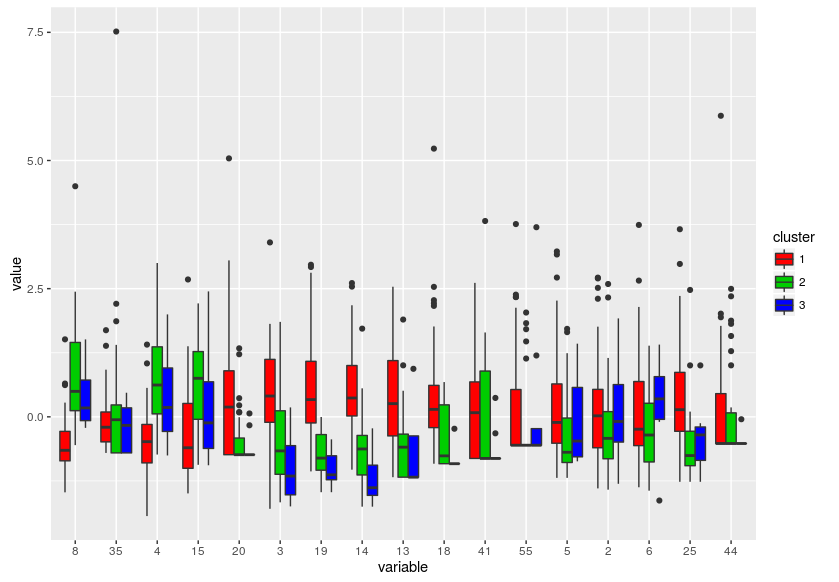
\includegraphics[width=0.5\textwidth]{cluster_whiskers}
	\caption{Whiskers plots in the most relevant features (time-based)}
	\label{fig:whiskers}
\end{figure}


\section{Conclusions}
The goal of is paper was to shed some light on what would be a proper method to characterise discussions online forums. For that, we analysed three different kinds of neighbourhood applicable to tree structures by which conversation threads are represented. We named this three types of neighbourhood structure-based, order-based and time-based. While the first one is a mere extension of the classical concept of neighbourhood in a graph, the aim of the other two is to explicitly consider time when deciding which are the neighbours of a given post.

We showed the limitations of the order-based to capture the structure of conversations. We think this finding is relevant because, in some contexts, order is more relevant than real time, and assuming that posts (or whatever vertices represent) arrive in homogeneous intervals gives excellent results \cite{Gomez2012}. 

In the context of online discussions, time is critical and must be considered in the definition of the neighbourhood motifs. Our choice has been to use \textit{changepoints}, variations in the pace of the discussion, to decide where a neighbourhood ends. Besides explicitly considering time, this method gives in practice relatively small neighbourhoods, which guarantees its scalability since isomorphisms are considerably fast to compute in small graphs.  

We also showed that, thanks to the use of changepoints to set limits of the neighbourhoods, the space of neighbourhoods is considerably reduced with respect to the structural neighbourhood. 

Finally, we used this neighbourhoods to characterise users in terms of the structure of the conversations they participate in and showed that, indeed, there are different types of structural conversationalists.

%Future
The concept of structural-temporal neighbourhood opens the door to some interesting paths of research.  The space of neighbourhoods is still quite large and, besides using pruning strategies more aggressive, it would be interesting to analyse which neighbourhoods, despite of being non-isomorphic, may represent the same type of conversation. Such analyse would allow to merge some of the neighbourhoods resulting in an even more reduced and meaningful space. Also, other kind of neighbourhoods can also be studied to analyse different phenomena. For instance, we might take only those neighbours which are descendants of the ego post. Such kind of neighbourhood may be used to classify users in terms in the reaction they trigger in the discussion. The inverse technique, that is, take all the neighbours that are not descendants of the ego, may help to understand the kind of discussion that a users tends to be attracted to. This might be useful for posts recommendations or even to improve current generative models that try to reproduce the way how a thread grows \cite{Gomez2012, Kumar2010}.


\begin{figure*}
	\centering
	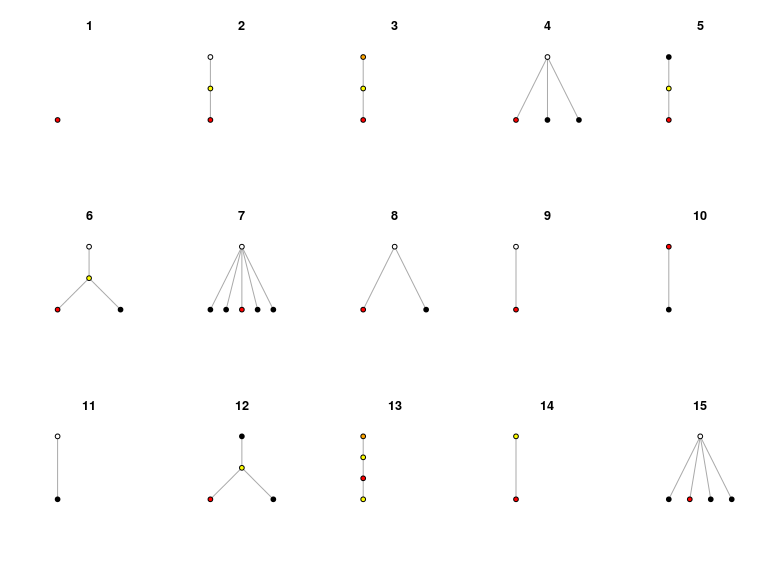
\includegraphics[width=0.8\textwidth]{dictionary1}
	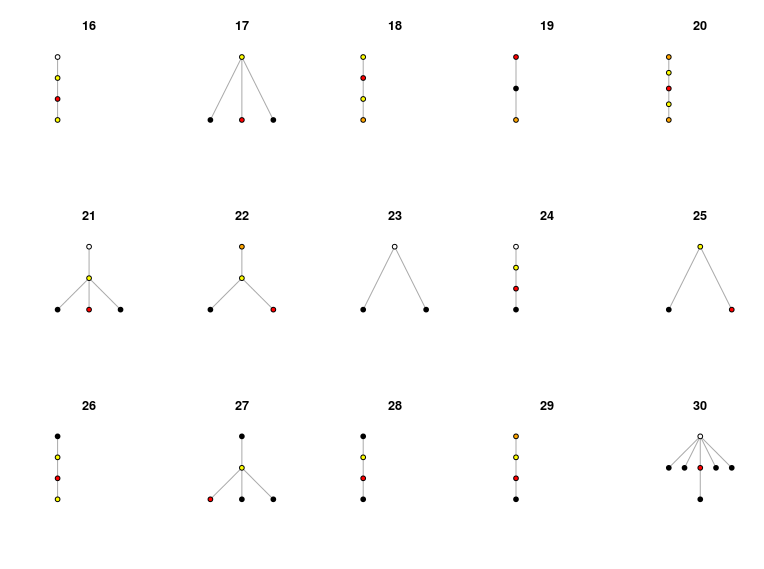
\includegraphics[width=0.8\textwidth]{dictionary2}
	\caption{Neighbourhoods reference list}
	\label{fig:dictionary}
\end{figure*}


% use section* for acknowledgment
%\section*{Acknowledgment}

% trigger a \newpage just before the given reference
% number - used to balance the columns on the last page
% adjust value as needed - may need to be readjusted if
% the document is modified later
%\IEEEtriggeratref{8}
% The "triggered" command can be changed if desired:
%\IEEEtriggercmd{\enlargethispage{-5in}}


\bibliographystyle{IEEEtran}
\bibliography{bibliography}

% that's all folks
\end{document}


